\section{Hierarchization on Full Grids (Unidirectional Principle)}
\label{sec:42fullGrids}

If $\sgset$ is a full grid $\fgset{\*l}$
(see \cref{sec:21nodalSpaces}),
the well-known \up
can be used to apply $\linop$ to input data $\vlinin$.
As shown in \cref{fig:unidirectionalPrinciple} for a sparse grid,
the idea of the \up
is to apply the corresponding one-dimensional operators on the
one-dimensional subgrids (the \term{poles}) of $\sgset$,
which is repeated for all dimensions.
In this section, we first formulate the \up for
general linear operators $\linop$ and then prove its correctness for
the case $\linop = \intpmatinv$ of hierarchization.
The correctness for arbitrary tensor product operators
will follow from \cref{sec:45spatAdaptiveUP}.

\begin{figure}
  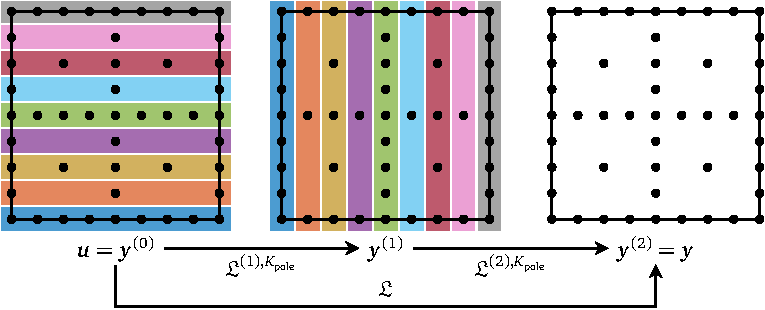
\includegraphics{unidirectionalPrinciple_1}%
  \caption[%
    Unidirectional principle%
  ]{%
    Application of a linear operator $\linop$
    on two-dimensional sparse grid data with the unidirectional principle.
    \emph{Left:}
    The univariate operator $\upopuv{1}{\lisetpole}$ is applied on
    the input data $\vlinin$
    along poles $\lisetpole$ of the first dimension $x_1$.
    \vspace{-0.2em}%
    \emph{Center:}
    The univariate operator $\upopuv{2}{\lisetpole}$ is applied on the
    resulting intermediate data $\vlinout[(1)]$
    along poles $\lisetpole$ of the second dimension $x_2$.
    \emph{Right:}
    Final values $\vlinout = \linop[\vlinin]$ after the application
    on both dimensions.
    All grid points of the same color are part of the same pole $\lisetpole$
    (equivalence classes of $\samepole{t}$ in
    \cref{alg:unidirectionalPrinciple}).%
  }%
  \label{fig:unidirectionalPrinciple}%
\end{figure}

\paragraph{Unidirectional principle and its correctness}

We state the \up in \cref{alg:unidirectionalPrinciple}.
The algorithm is given a permutation $(t_1, \dotsc, t_d)$ of $(1, \dotsc, d)$
that specifies the order of dimensions in which the \up should be applied.
We denote with $\upopuv{t_j}{\lisetpole}$ the one-dimensional version of $\linop$
applied in dimension $t_j$ ($j = 1, \dotsc, d$) on the pole $\lisetpole$.
Formally, a pole is an equivalence class of the
\term{pole equivalence relation} $\samepole{t_j}$ on $\liset$:
\begin{equation}
  \label{eq:poleEquivalenceRelation}
  \*k' \samepole{t_j} \*k'' \iff \*k'_{-t_j} = \*k''_{-t_j},\quad
  \*k', \*k'' \in \liset.
\end{equation}
We prove the correctness of the \up with the following invariant:

\begin{algorithm}
  \begin{algorithmic}[1]
    \Function{$\vlinout = \texttt{unidirectionalPrinciple}$}{%
      $\vlinin$, $\liset$, $(t_1, \dotsc, t_d)$%
    }
      \State{$\vlinout[(0)] \gets \vlinin$}
      \For{$j = 1, \dotsc, d$}
        \For{$\lisetpole \in \eqclasses{\liset}{\samepole{t_j}}$}
          \State{%
            $(\linout[(j)]{\*k})_{\*k \in \lisetpole} \gets
            \upopuv{t_j}{\lisetpole}
            \bracket*{(\linout[(j-1)]{\*k})_{\*k \in \lisetpole}}$%
          }
          \Comment{apply univariate operator on pole}%
          \label{line:algUnidirectionalPrinciple1}
        \EndFor{}
      \EndFor{}
      \State{$\vlinout \gets \vlinout[(d)]$}
    \EndFunction{}
  \end{algorithmic}
  \caption[%
    Unidirectional principle%
  ]{%
    Application of a tensor product operator $\linop$ with
    the unidirectional principle.
    Inputs are
    the vector $\vlinin = (\linin{\*k})_{\*k \in \liset}$ of input data,
    the set $\liset$ of grid indices, and
    the permutation $(t_1, \dotsc, t_d)$ specifying the order in which
    the one-dimensional operators $\upopuv{t_j}{\lisetpole}$ should be applied.
    The output is the vector $\vlinout = (\linout{\*k})_{\*k \in \liset}$
    of output data.%
  }%
  \label{alg:unidirectionalPrinciple}%
\end{algorithm}

\begin{proposition}[invariant of unidirectional principle for hierarchization]
  \label{prop:invariantUnidirectionalPrinciple}
  Let $\linop$ be the hierarchization operator on a full grid,
  i.e.,
  $\linop = \intpmatinv$,
  $\vlinin = (\fcnval{\*k})_{\*k \in \liset}$,
  $\vlinout = (\surplus{\*k})_{\*k \in \liset}$,
  $\upopuv{t_j}{\lisetpole}$ is the univariate interpolation operator
  $\intpmatuvinv{t_j}$, and
  $\liset = \{\*0, \dotsc, \*2^\*l\}$
  corresponds to a full grid $\fgset{\*l}$ of level $\*l$.
  After iteration $j$ of \cref{alg:unidirectionalPrinciple}
  ($j = 1, \dotsc, d$), it holds for $T \ceq (t_1, \dotsc, t_j)$
  \begin{equation}
    \sum_{\*k_T=\*0}^{\*2^{\*l_T}}
    \linout[(j)]{(\*k_T,\*k'_{-T})} \basis{\*k_T}(\gp{\*k'_T})
    = \fcnval{\*k'},\quad
    \*k' = \*0, \dotsc, \*2^\*l,
  \end{equation}
  where $(\*k_T,\*k'_{-T})$ is shorthand for $\*k''$
  with $k''_t \ceq k_t$ if $t \in T$ and $k''_t \ceq k'_t$ if $t \notin T$.
\end{proposition}

\begin{proof}
  We prove the assertion by induction over $j = 1, \dotsc, d$.
  We set $T' \ceq (t_1, \dotsc, t_{j-1})$,
  $T \ceq (t_1, \dotsc, t_{j-1}, t_j)$,
  and we exploit the tensor product structure of the basis
  to write the \lhs of the assertion for $j$
  and arbitrary $\*k' = \*0, \dotsc, \*2^\*l$ as
  \begin{equation}
    \label{eq:proofPropInvariantUnidirectionalPrinciple1}
    \sum_{\*k_T=\*0}^{\*2^{\*l_T}}
    \linout[(j)]{(\*k_T,\*k'_{-T})} \basis{\*k_T}(\gp{\*k'_T})
    = \sum_{\*k_{T'}=\*0}^{\*2^{\*l_{T'}}}
    \basis{\*k_{T'}}(\gp{\*k'_{T'}})
    \sum_{k_{t_j}=0}^{2^{l_{t_j}}}
    \linout[(j)]{(\*k_T,\*k'_{-T})} \basis{k_{t_j}}(\gp{k'_{t_j}}).
  \end{equation}
  If we choose the equivalence class
  $\lisetpole \ceq \eqclass{(\*k_T,\*k'_{-T})}{\samepole{t_j}}$
  ($\*k_T$ arbitrary),
  then the inner sum over $k_{t_j}$ equals
  \begin{equation}
    \label{eq:proofPropInvariantUnidirectionalPrinciple2}
    \sum_{\*k'' \in \lisetpole}
    \linout[(j)]{\*k''} \basis{k''_{t_j}}(\gp{k'_{t_j}})
    = \paren*{
      (\upopuv{t_j}{\lisetpole})^{-1}
      \bracket*{(\linout[(j)]{\*k''})_{\*k'' \in \lisetpole}}
    }_{k'_{t_j}}
    = \linout[(j-1)]{(\*k_{T'},\*k'_{-T'})}
  \end{equation}
  by \cref{line:algUnidirectionalPrinciple1} of
  \cref{alg:unidirectionalPrinciple}.
  We can conclude that the \lhs
  \cref{eq:proofPropInvariantUnidirectionalPrinciple1} equals
  \begin{equation}
    \sum_{\*k_{T'}=\*0}^{\*2^{\*l_{T'}}}
    \linout[(j-1)]{(\*k_{T'},\*k'_{-T'})}
    \basis{\*k_{T'}}(\gp{\*k'_{T'}}),
  \end{equation}
  which, by the induction hypothesis, equals $\fcnval{\*k'}$ as desired
  (if $j > 1$).
  The same reasoning for
  \eqref{eq:proofPropInvariantUnidirectionalPrinciple2} can be used
  to establish the base case for $j = 1$.
\end{proof}

\begin{shortcorollary}[%
  correctness of unidirectional principle for hierarchization%
]
  \label{cor:algUnidirectionalPrincipleCorrectness}
  \Cref{alg:unidirectionalPrinciple}
  is correct for hierarchization on full grids.
\end{shortcorollary}

\begin{proof}
  We apply \cref{prop:invariantUnidirectionalPrinciple} for $j = d$ to obtain
  $\sum_{\*k=\*0}^{\*2^\*l}
  \linout[(j)]{\*k} \basis{\*k}(\gp{\*k'})
  = \fcnval{\*k'}$
  for all $\*k' = \*0, \dotsc, \*2^\*l$, i.e.,
  the $\linout[(j)]{\*k}$ are the correct interpolation coefficients
  according to \eqref{eq:hierarchizationProblem}.
\end{proof}

\paragraph{Complexity}

We compare the complexity of the \up for hierarchization with
the direct solution of the system \eqref{eq:hierarchizationSLE} of
linear equations.
If we assume that $d$ is constant and that
$\linop$ and $\upopuv{t_j}{\lisetpole}$ apply Gaussian elimination to
solve the multivariate and univariate systems, respectively,
then directly solving \eqref{eq:hierarchizationSLE} takes
$\landauO{\ngp^2 (\ngp + d)}$ time and
$\landauO{\ngp^2}$ memory.
In contrast, the \up only requires
$\landauO{\ngp \sum_t \ngp_t^2}$ time%
\footnote{%
  There are $\ngp/\ngp_t$ poles in the
  $t$-th iteration of \cref{alg:unidirectionalPrinciple}.
  Each pole requires the solution of an $\ngp_t \times \ngp_t$ linear system,
  which takes $\landauO{\ngp_t^3}$ time.%
}
and $\landauO{\max\{N_1^2, \dotsc, N_d^2, N\}}$ memory,
where $\ngp_t$ is the grid size
$\setsize{\{k_t \mid \*k \in \liset\}}$ in dimension $t = 1, \dotsc, d$.
The dependency from the univariate grid sizes $\ngp_t$ instead of $\ngp$
makes the \up significantly less computationally expensive.
As already mentioned,
the \up is even more efficient in the piecewise linear case,
where the univariate interpolation operators can be applied
in-place.
Hence, it only needs $\landauO{Nd}$ time and
$\landauO{N}$ memory in this case.
